\documentclass{beamer}

\mode<presentation>{
    \usetheme{Madrid}
}

% XeLaTeX font configuration with full Vietnamese glyph coverage.
\usepackage{fontspec}
\setsansfont{Arial}
\setmonofont{Menlo}
\usepackage{amsmath,amsfonts,amssymb}
\usepackage{booktabs}
\usepackage{hyperref}
\usepackage{tikz}
\usepackage{xcolor}
\usepackage{graphicx}

\newcommand{\resultfigure}[2]{%
    \IfFileExists{#1}{%
        \includegraphics[width=0.85\textwidth,height=0.56\textheight,keepaspectratio]{#1}%
    }{%
        \begin{beamercolorbox}[wd=0.85\textwidth,ht=0.38\textheight,dp=0.04\textheight,center,rounded=true]{block body}%
            \small #2
        \end{beamercolorbox}%
    }%
}

\title[CĐNLP]{Phân tích độ bền vững của mô hình hỏi đáp hóa đơn tiếng Việt trước lỗi OCR}
\subtitle{Báo cáo tiến độ môn Chuyên đề Xử lý Ngôn ngữ Tự nhiên}
\author{Nhóm 19}
\institute[UIT]{Trường Đại học Công nghệ Thông tin \\ Đại học Quốc gia TP.HCM}
\date{\today}

\begin{document}

\begin{frame}
    \titlepage
\end{frame}

\section{Bài toán}

\begin{frame}
\frametitle{Bài toán nghiên cứu}

\begin{center}
\textbf{Câu hỏi + OCR hóa đơn -> đáp án ngắn}
\end{center}

\vspace{0.25cm}
\begin{columns}[T,onlytextwidth]
\begin{column}{0.48\textwidth}
\begin{block}{Đầu vào}
Câu hỏi tiếng Việt\\
Văn bản OCR của hóa đơn
\end{block}
\end{column}
\begin{column}{0.48\textwidth}
\begin{block}{Đầu ra}
Tổng tiền\\
Ngày, cửa hàng, địa chỉ
\end{block}
\end{column}
\end{columns}

\vspace{0.2cm}
\begin{alertblock}{Câu hỏi trọng tâm}
OCR nhiễu làm ANLS giảm bao nhiêu, và huấn luyện với nhiễu có giúp giảm mức suy giảm không?
\end{alertblock}

\end{frame}

\begin{frame}
\frametitle{Ví dụ lỗi OCR trên hóa đơn}

\begin{columns}[T,onlytextwidth]
\begin{column}{0.28\textwidth}
\centering
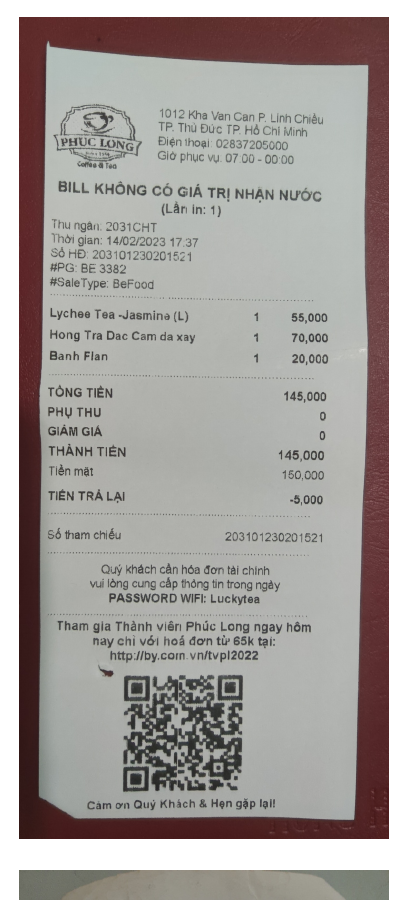
\includegraphics[height=0.52\textheight,keepaspectratio]{img/illustrations/receiptvqa_sample_upper_v3.png}

\scriptsize Ví dụ hóa đơn trong ReceiptVQA
\end{column}

\begin{column}{0.68\textwidth}
\textbf{OCR sạch}
\begin{itemize}
    \item Tổng cộng: 125.000đ
    \item Ngày bán: 01/02/2024
\end{itemize}

\textbf{OCR nhiễu}
\begin{itemize}
    \item Tong cong: 125 OOO d
    \item Ngay ban: O1/O2/2O24
\end{itemize}

\begin{alertblock}{Rủi ro với câu hỏi ``Tổng số tiền là bao nhiêu?''}
Sai số, ký tự và định dạng tiền có thể làm đáp án sai.
\end{alertblock}
\end{column}
\end{columns}

\vspace{0.08cm}
\tiny Nguồn hình: Le et al. (2025), Fig. 1, ReceiptVQA.

\end{frame}

\section{Mục tiêu}

\begin{frame}
\frametitle{Mục tiêu và câu hỏi nghiên cứu}

\begin{enumerate}
    \item Baseline ViT5 trên OCR sạch
    \item 14 nhiễu OCR có kiểm soát tại L2
    \item So sánh Noisy Aug và Consistency
\end{enumerate}

\vspace{0.18cm}
\begin{block}{Ba câu hỏi}
Nhiễu nào hại nhất? \quad Noisy Aug có giúp không? \quad Consistency đổi clean/noisy ra sao?
\end{block}

\scriptsize Phạm vi: ViT5, một seed, synthetic OCR noise tại L2.

\end{frame}

\section{Dữ liệu}

\begin{frame}
\frametitle{Dữ liệu ReceiptVQA}

\begin{columns}[T,onlytextwidth]
\begin{column}{0.62\textwidth}
\begin{table}
\centering
\begin{tabular}{lr}
\toprule
\textbf{Thành phần} & \textbf{Số lượng} \\
\midrule
Ảnh hóa đơn/OCR & 9.500 \\
Train QA & 51.886 \\
Dev QA & 6.426 \\
Test QA & 6.500 \\
\bottomrule
\end{tabular}
\end{table}

\begin{block}{Dữ liệu đã kiểm tra}
Split gốc ReceiptVQA \quad 9.500 OCR features
\end{block}
\end{column}

\begin{column}{0.34\textwidth}
\centering
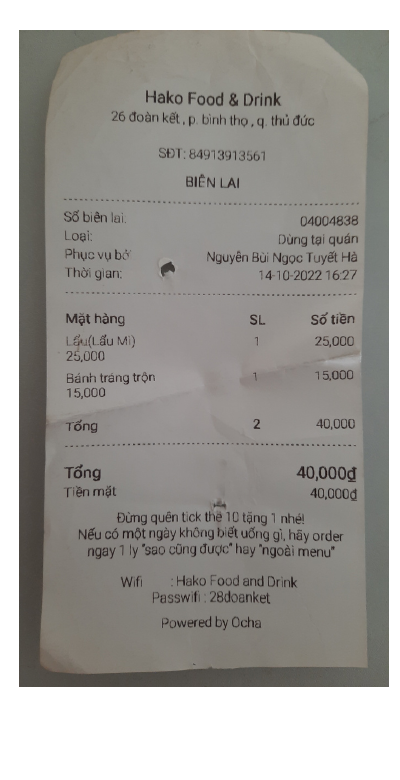
\includegraphics[height=0.48\textheight,keepaspectratio]{img/illustrations/receiptvqa_sample_lower_v3.png}

\scriptsize Mẫu ReceiptVQA
\end{column}
\end{columns}

\vspace{0.06cm}
\tiny Nguồn hình: Le et al. (2025), Fig. 1, ReceiptVQA.

\end{frame}

\section{Phương pháp}

\begin{frame}
\frametitle{Pipeline thực nghiệm}

\begin{center}
\begin{tikzpicture}[node distance=1.2cm, every node/.style={font=\small}]
\node[draw, rounded corners, fill=blue!12, minimum width=3.2cm] (data) {ReceiptVQA};
\node[draw, rounded corners, fill=green!12, below of=data, minimum width=3.2cm] (clean) {OCR sạch};
\node[draw, rounded corners, fill=orange!15, right of=clean, xshift=3.2cm, minimum width=3.4cm] (noise) {Sinh OCR nhiễu};
\node[draw, rounded corners, fill=purple!12, below of=clean, yshift=-0.1cm, minimum width=3.6cm] (base) {Train ViT5 baseline};
\node[draw, rounded corners, fill=red!12, below of=noise, yshift=-0.1cm, minimum width=4.4cm, align=center] (aug) {Train ViT5 robust\\(Noisy Aug / Consistency)};
\node[draw, rounded corners, fill=gray!15, below of=base, xshift=2.9cm, yshift=-0.1cm, minimum width=4.8cm] (eval) {Đánh giá clean/noisy ANLS};

\draw[->] (data) -- (clean);
\draw[->] (clean) -- (noise);
\draw[->] (clean) -- (base);
\draw[->] (noise) -- (aug);
\draw[->] (base) -- (eval);
\draw[->] (aug) -- (eval);
\end{tikzpicture}
\end{center}

\vspace{0.2cm}

\textbf{So sánh:} 3 phương pháp \quad 14 nhiễu \quad cùng test set tại L2

\end{frame}

\begin{frame}
\frametitle{Bộ 14 loại nhiễu OCR}

\begin{columns}[T,onlytextwidth]
\begin{column}{0.48\textwidth}
\begin{block}{Sai ký tự \quad 6 loại}
Mất dấu \quad đổi dấu \quad đ/d\\
0/O, 1/l \quad glyph giống nhau
\end{block}
\begin{block}{Mất thông tin \quad 2 loại}
Xóa ký tự \quad xóa token
\end{block}
\end{column}
\begin{column}{0.48\textwidth}
\begin{block}{Cấu trúc \quad 2 loại}
Đảo dòng \quad tách token
\end{block}
\begin{block}{Trường quan trọng \quad 4 loại}
Tiền \quad ngày \quad mã \quad mixed noise
\end{block}
\end{column}
\end{columns}

\vspace{0.15cm}
\begin{center}
\texttt{125.000đ -> 125 OOO d} \qquad \texttt{01/02/2024 -> O1/O2/2O24}
\end{center}


\end{frame}

\section{Thiết lập}

\begin{frame}
\frametitle{Thiết lập thực nghiệm hiện tại}

\begin{columns}[T,onlytextwidth]
\begin{column}{0.48\textwidth}
\begin{block}{Mô hình}
ViT5-base\\
Input 256 \quad Output 64\\
Beam search $k=4$
\end{block}
\end{column}
\begin{column}{0.48\textwidth}
\begin{block}{Huấn luyện}
Full data \quad 3 epochs\\
Learning rate $5 \times 10^{-5}$\\
ANLS, threshold 0.5
\end{block}
\end{column}
\end{columns}

\vspace{0.2cm}
\begin{alertblock}{Kiểm soát}
Seed noise = 42 \quad cùng test set \quad synthetic OCR noise tại L2
\end{alertblock}

\end{frame}

\section{Tiến độ}

\begin{frame}
\frametitle{Tiến độ thực hiện}

\begin{center}
\textbf{3 phương pháp \qquad 14 nhiễu \qquad 1 benchmark L2}
\end{center}

\vspace{0.45cm}
\begin{columns}[T,onlytextwidth]
\begin{column}{0.48\textwidth}
\begin{block}{Đã hoàn thành}
Dataset và loader\\
Taxonomy nhiễu\\
Huấn luyện và đánh giá
\end{block}
\end{column}
\begin{column}{0.48\textwidth}
\begin{block}{Đầu ra đã lưu}
CSV cho 3 flow\\
Ranking noise\\
Biểu đồ recovery
\end{block}
\end{column}
\end{columns}

\end{frame}
\section{Kết quả thực nghiệm}

\begin{frame}
\frametitle{Kết quả chính trên ReceiptVQA }

\begin{center}
\resultfigure{img/fig_method_summary.png}{Biểu đồ tổng hợp phương pháp chưa có trong workspace.}
\end{center}

\begin{alertblock}{Kết quả chính}
\textbf{Noisy Aug cao nhất:} 85.34 clean \quad 84.23 noisy \quad drop 1.11
\end{alertblock}

\scriptsize Lưu ý: Noisy Aug dùng clean $N$ + noisy $N$, gần gấp đôi dữ liệu/updates so với baseline.

\end{frame}

\begin{frame}
\frametitle{Ranking mức ảnh hưởng tại L2}

\begin{center}
\resultfigure{img/fig_noise_drop_ranking.png}{Biểu đồ xếp hạng mức suy giảm theo 14 loại nhiễu chưa có trong workspace.}
\end{center}

\vspace{0.1cm}
\begin{center}
\textbf{mixed noise: $-9.88$} \qquad \textbf{money noise: $-4.99$}
\end{center}

\scriptsize Một lần chạy L2 của ViT5 baseline; cần confidence interval để kết luận chênh lệch nhỏ.

\end{frame}

\begin{frame}
\frametitle{Vì sao money noise nguy hiểm?}

\begin{center}
\resultfigure{img/fig_answer_distribution.png}{Biểu đồ phân phối loại câu trả lời chưa có trong workspace.}
\end{center}

\vspace{0.1cm}
\begin{center}
\textbf{$\sim$49\% đáp án là số/số điện thoại}
\end{center}

\scriptsize Sai một ký tự ở đáp án ngắn có thể đẩy ANLS dưới ngưỡng 0.5.

\end{frame}

\begin{frame}
\frametitle{money\_noise vs date\_noise: khác 27 lần}

\begin{block}{Cùng xác suất p = 0.30, khác mức hại}
money: $-4.99$ \qquad date: $-0.19$ \qquad \textbf{chênh 27$\times$}
\end{block}

\vspace{0.2cm}

\begin{table}
\small
\centering
\begin{tabular}{lccc}
\toprule
\textbf{Field} & \textbf{\% answer khớp} & \textbf{Drop} & \textbf{Drop / \%exposure} \\
\midrule
money/number & 48.75\% & $-4.99$ & 0.102 \\
date & 5.22\% & $-0.19$ & 0.036 \\
\bottomrule
\end{tabular}
\end{table}

\vspace{0.2cm}

\scriptsize Tỷ lệ xuất hiện trong gold answer chỉ là proxy. Cần phân tích từng mẫu OCR để kiểm tra nguyên nhân.

\end{frame}

\begin{frame}
\frametitle{So sánh khả năng phục hồi: Noisy Aug vs Consistency}

\begin{center}
\resultfigure{img/fig_recovery.png}{Biểu đồ phục hồi của Noisy Aug và Consistency chưa có trong workspace.}
\end{center}

\vspace{0.1cm}
\begin{center}
\textbf{Noisy Aug cao hơn Consistency ở 14 điều kiện L2}
\end{center}

\scriptsize So sánh còn chịu ảnh hưởng bởi ngân sách train không bằng nhau.

\end{frame}

\begin{frame}
\frametitle{Vì sao Consistency không vượt được Noisy Aug?}

\begin{columns}[T,onlytextwidth]
\begin{column}{0.47\textwidth}
\begin{block}{Noisy Aug}
Clean/noisy là mẫu độc lập\\
Tối ưu cross-entropy
\end{block}
\end{column}
\begin{column}{0.47\textwidth}
\begin{block}{Consistency}
Thêm $h_{clean} \approx h_{noisy}$\\
Cosine trên mean-pool
\end{block}
\end{column}
\end{columns}

\vspace{0.25cm}
\begin{alertblock}{Quan sát}
Consistency: clean 83.97, thấp hơn baseline 0.14. Giả thuyết: over-regularization.
\end{alertblock}

\scriptsize Cần equal-budget run và confidence interval.

\end{frame}
\begin{frame}
\frametitle{Kế hoạch tiếp theo}

\begin{enumerate}
    \item Equal-budget run cho baseline và Noisy Aug
    \item Lưu prediction từng mẫu, bootstrap CI
    \item Phân tích money/mixed trên OCR context bị ảnh hưởng
\end{enumerate}

\begin{alertblock}{Giới hạn cần giữ}
Synthetic noise, một seed, L2. Chưa đánh giá OCR engine thực.
\end{alertblock}

\end{frame}



\begin{frame}
\frametitle{Hướng mở rộng}

\begin{table}
\small
\centering
\begin{tabular}{lll}
\toprule
\textbf{TN} & \textbf{Phương pháp} & \textbf{Mục tiêu kiểm tra} \\
\midrule
4 & Adapter Only & Giảm số tham số huấn luyện, giữ nền ViT5 cố định \\
5 & RON-NACA & Kết hợp adapter và consistency loss \\
\bottomrule
\end{tabular}
\end{table}

\vspace{0.2cm}

\begin{block}{Mục tiêu}
Adapter Only: ít tham số cập nhật\\
RON-NACA: adapter + consistency
\end{block}

\textbf{Trạng thái:} chưa chạy. Thực hiện sau equal-budget run và confidence interval.

\end{frame}

\begin{frame}
\frametitle{Đóng góp}

\begin{enumerate}
    \item Benchmark ViT5 trên full ReceiptVQA
    \item 14 nhiễu OCR có kiểm soát tại L2
    \item Noisy Aug đạt ANLS tuyệt đối cao nhất trong lần chạy này
\end{enumerate}

\begin{block}{Thông điệp chính}
Đánh giá độ bền OCR có kiểm soát; kết luận cần equal-budget run và confidence interval.
\end{block}

\end{frame}

\begin{frame}
\begin{center}
\Huge{Cảm ơn!}

\vspace{1cm}

\Large{Câu hỏi và thảo luận}
\end{center}
\end{frame}

\end{document}
